\documentclass[tikz,border=8pt]{standalone}
% Shared look for every TikZ diagram. Load with \input{../../tools/tikz-style.tex}
\usepackage[sfdefault]{roboto}
\usetikzlibrary{arrows.meta, positioning, shapes.geometric, calc, fit, backgrounds}
\definecolor{cblue}{HTML}{4C78A8}
\definecolor{corange}{HTML}{F58518}
\definecolor{cgreen}{HTML}{54A24B}
\definecolor{cred}{HTML}{E45756}
\definecolor{cpurple}{HTML}{B279A2}
\definecolor{cgrey}{HTML}{6B6B6B}
\tikzset{
  every picture/.style={font=\sffamily, line width=1.2pt},
  box/.style={draw=#1, fill=#1!12, rounded corners=4pt, align=center, inner sep=7pt, minimum height=1.1cm},
  box/.default=cgrey,
  arrow/.style={-{Stealth[length=3mm]}, draw=cgrey, line width=1.4pt},
  title/.style={font=\sffamily\bfseries\Large},
  note/.style={font=\sffamily\small, text=cgrey, align=center},
}
\AtBeginDocument{\hyphenpenalty=10000 \exhyphenpenalty=10000}

% History and depth (ROS 2 docs, Quality of Service settings): keep last N stores up to N messages; keep all stores
% every message. The planner is busy from 2.4 s to 2.7 s while scans arrive every 0.1 s.
\begin{document}
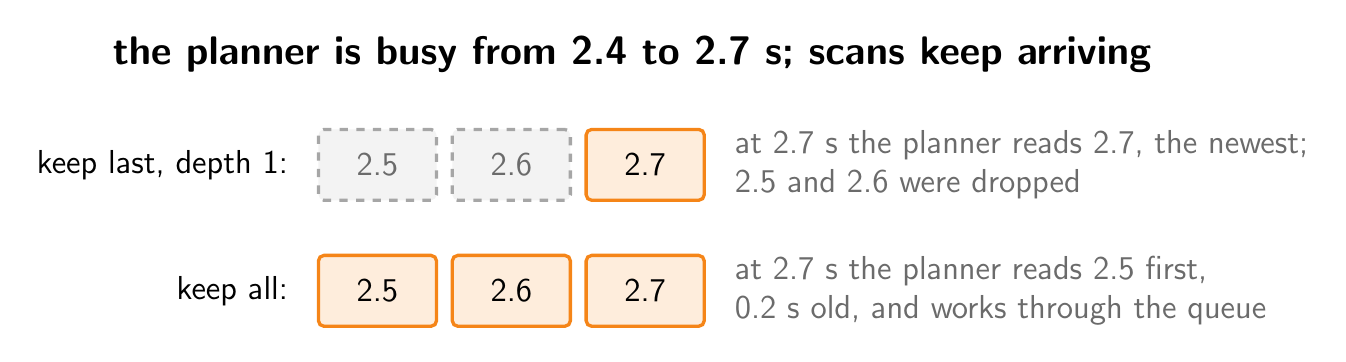
\begin{tikzpicture}[sc/.style={draw=corange, fill=corange!15, rounded corners=2pt, font=\sffamily\large, minimum width=1.5cm, minimum height=0.9cm},
  dr/.style={draw=cgrey!60, fill=cgrey!8, dashed, rounded corners=2pt, font=\sffamily\large, text=cgrey, minimum width=1.5cm, minimum height=0.9cm}]
  \node[title, anchor=west] at (-0.3,2.4) {the planner is busy from 2.4 to 2.7 s; scans keep arriving};
  \node[font=\sffamily\large, anchor=east] at (2.2,1.0) {keep last, depth 1:};
  \node[dr] at (3.2,1.0) {2.5}; \node[dr] at (4.9,1.0) {2.6}; \node[sc] at (6.6,1.0) {2.7};
  \node[note, font=\sffamily\large, anchor=west, align=left] at (7.6,1.0) {at 2.7 s the planner reads 2.7, the newest;\\ 2.5 and 2.6 were dropped};
  \node[font=\sffamily\large, anchor=east] at (2.2,-0.6) {keep all:};
  \node[sc] at (3.2,-0.6) {2.5}; \node[sc] at (4.9,-0.6) {2.6}; \node[sc] at (6.6,-0.6) {2.7};
  \node[note, font=\sffamily\large, anchor=west, align=left] at (7.6,-0.6) {at 2.7 s the planner reads 2.5 first,\\ 0.2 s old, and works through the queue};
\end{tikzpicture}
\end{document}
